% !TEX TS-program = xelatex
% !BIB program = bibtex
% !TeX spellcheck = ru_RU

% About magic macros see also
% https://tex.stackexchange.com/questions/78101/

% По умолчанию используется шрифт 14 размера.
% Если Вы не влезаете в лимит страниц и нужен 12-й шрифт,
% то уберите опцию [14pt]

\documentclass[14pt, russian]{matmex-diploma-custom}


% !TeX spellcheck = ru_RU
% !TEX root = vkr.tex
% Опциональные добавления используемых пакетов. Вполне может быть, что они вам не понадобятся, но в шаблоне приведены примеры их использования.
\usepackage{tikz} % Мощный пакет для создание рисунков, однако может очень сильно замедлять компиляцию
\usetikzlibrary{decorations.pathreplacing,calc,shapes,positioning,tikzmark}

% Библиотека для TikZ, которая генерирует отдельные файлы для каждого рисунка
% Позволяет ускорить компиляцию, однако имеет свои ограничения
% Например, ломает пример выделения кода в листинге из шаблона
% \usetikzlibrary{external}
% \tikzexternalize[prefix=figures/]

\newcounter{tmkcount}

\tikzset{
    use tikzmark/.style={
            remember picture,
            overlay,
            execute at end picture={
                    \stepcounter{tmkcount}
                },
        },
    tikzmark suffix={-\thetmkcount}
}

\usepackage{booktabs} % Пакет для верстки "более книжных" таблиц, вполне годится для оформления результатов
% В шаблоне есть команда \multirowcell, которой нужен этот пакет.
\usepackage{multirow}
\usepackage{siunitx} % для таблиц с единицами измерений

% Для названий стоит использовать \textsc{}
\newcommand{\OCaml}{\textsc{OCaml}}
\newcommand{\miniKanren}{\textsc{miniKanren}}
\newcommand{\BibTeX}{\textsc{BibTeX}}
\newcommand{\vsharp}{\textsc{V$\sharp$}}
\newcommand{\fsharp}{\textsc{F$\sharp$}}
\newcommand{\csharp}{\textsc{C\#}}
\newcommand{\GitHub}{\textsc{GitHub}}
\newcommand{\SMT}{\textsc{SMT}}

\definecolor{eclipseGreen}{RGB}{63,127,95}
% \lstdefinelanguage{ocaml}{
% keywords={@type, function, fun, let, in, match, with, when, class, type,
% nonrec, object, method, of, rec, repeat, until, while, not, do, done, as, val, inherit, and,
% new, module, sig, deriving, datatype, struct, if, then, else, open, private, virtual, include, success, failure,
% lazy, assert, true, false, end},
% sensitive=true,
% commentstyle=\small\itshape\ttfamily,
% keywordstyle=\ttfamily\bfseries, %\underbar,
% identifierstyle=\ttfamily,
% basewidth={0.5em,0.5em},
% columns=fixed,
% fontadjust=true,
% literate={->}{{$\to$}}3 {===}{{$\equiv$}}1 {=/=}{{$\not\equiv$}}1 {|>}{{$\triangleright$}}3 {\\/}{{$\vee$}}2 {/\\}{{$\wedge$}}2 {>=}{{$\ge$}}1 {<=}{{$\le$}} 1,
% morecomment=[s]{(*}{*)}
% }

\makeatletter
\@ifclassloaded{beamer}{
    %%% Обязательные пакеты
    %% Beamer
    \usepackage{beamerthemesplit}
    \usetheme{SPbGU}
    \beamertemplatenavigationsymbolsempty
    \usepackage{appendixnumberbeamer}

    %% Локализация
    \usepackage{fontspec}
    \setmainfont{CMU Serif}
    \setsansfont{CMU Sans Serif}
    \setmonofont{CMU Typewriter Text}
    %\setmonofont{Fira Code}[Contextuals=Alternate,Scale=0.9]
    %\setmonofont{Inconsolata}
    \usepackage{polyglossia}
    \setmainlanguage{russian}
    \setotherlanguage{english}

    %% Графика
    \usepackage{pdfpages} % Позволяет вставлять многостраничные pdf документы в текст

    % Математические окружения с русским названием
    \newtheorem{rutheorem}{Теорема}
    \newtheorem{ruproof}{Доказательство}
    \newtheorem{rudefinition}{Определение}
    \newtheorem{rulemma}{Лемма}
    \usepackage{fancyvrb}
}
{}
\makeatother

\usepackage[autostyle]{csquotes} % Правильные кавычки в зависимости от языка
\usepackage{totcount}
\usepackage{setspace}
\usepackage{amsmath, amsfonts, amssymb, amsthm, mathtools} % "Адекватная" работа с математикой в LaTeX



\begin{document}

% !TeX spellcheck = ru_RU
% !TEX root = vkr.tex


%% Если что-то забыли, при компиляции будут ошибки Undefined control sequence \my@title@<что забыли>@ru
%% Если англоязычная титульная страница не нужна, то ее можно просто удалить.
\filltitle{ru}{
    date = {27 марта 2025},
    %% Актуально только для курсовых/практик. ВКР защищаются не на кафедре а в ГЭК по направлению,
    %%   и к моменту защиты вы будете уже не в группе.
    chair              = {Программная инженерия},
    group              = {24.М71-мм},
    %
    %% Макрос filltitle ненавидит пустые строки, поэтому обязателен хотя бы символ комментария на строке
    %% Актуально всем.
    title              = {Оценка проекта},
    %
    %% Здесь указывается тип работы. Возможные значения:
    %%   production - производственная практика;
    %%   coursework - отчёт по курсовой работе (ОБРАТИТЕ ВНИМАНИЕ, у техпрога и ПИ нет курсовых, только практики);
    %%   practice - отчёт по учебной практике;
    %%   prediploma - отчёт по преддипломной практике;
    %%   master - ВКР магистра;
    %%   bachelor - ВКР бакалавра.
    type               = {groupwork},
    %
    %% Здесь указывается вид работы. От вида работы зависят критерии оценивания.
    %%   solution - «Решение». Обучающемуся поручили найти способ решения проблемы в области разработки программного обеспечения или теоретической информатики с учётом набора ограничений.
    %%   experiment - «Эксперимент». Обучающемуся поручили изучить возможности, достоинства и недостатки новой технологии, платформы, языка и т. д. на примере какой-то задачи.
    %%   production - «Производственное задание». Автору поручили реализовать потенциально полезное программное обеспечение.
    %%   comparison - «Сравнение». Обучающемуся поручили сравнить несколько существующих продуктов и/или подходов.
    %%   theoretical - «Теоретическое исследование». Автору поручили доказать какое-то утверждение, исследовать свойства алгоритма и т.п., при этом не требуя написания кода.
    kind               = {none},
    %
    author             = {Juniors},
    %
    %% Актуально только для ВКР. Указывается код и название направления подготовки. Типичные примеры:
    %%   02.03.03 \enquote{Математическое обеспечение и администрирование информационных систем}
    %%   02.04.03 \enquote{Математическое обеспечение и администрирование информационных систем}
    %%   09.03.04 \enquote{Программная инженерия}
    %%   09.04.04 \enquote{Программная инженерия}
    %% Те, что с 03 в середине --- бакалавриат, с 04 --- магистратура.
    specialty          = {09.04.04 \enquote{Математическое обеспечение и администрирование информационных систем}},
    %
    %% Актуально только для ВКР. Указывается шифр и название образовательной программы. Типичные примеры:
    %%   СВ.5162.2020 \enquote{Технологии программирования}
    %%   СВ.5080.2020 \enquote{Программная инженерия}
    %%   ВМ.5665.2022 \enquote{Математическое обеспечение и администрирование информационных систем}
    %%   ВМ.5666.2022 \enquote{Программная инженерия}
    %% Шифр и название программы можно посмотреть в учебном плане, по которому вы учитесь.
    %% СВ.* --- бакалавриат, ВМ.* --- магистратура. В конце --- год поступления (не обязательно ваш, если вы были в академе/вылетали).
    programme          = {ВМ.5666.2024 \enquote{Технологии программирования}},
    %
    %% Актуально всем.
    %% Должно умещаться в одну строчку, допускается использование сокращений, но без переусердствования,
    %% короткая строка с большим количеством сокращений выглядит странно
    %supervisorPosition = {проф. кафeдры системного программирования, д.ф.-м.н.,}, % Терехов А. Н.
    %supervisorPosition = {ст. преподаватель кафедры ИАС, к.~ф.-м.~н. (если есть),}, % Смирнов К. К.
    supervisorPosition = {},
    supervisor         = {},
    teacher            = {Тимохин Д. В.}
    %
    %% Актуально только для практик и курсовых. Если консультанта нет или он совпадает с научником, закомментировать или удалить вовсе.
    % consultantPosition = {должность, ООО \enquote{Место работы}, степень  (если есть),},
    % consultant         = {Консультант~К.~К.},
    %
    %% Актуально только для ВКР.
    % reviewerPosition   = {должность, ООО \enquote{Место работы}, степень (если есть),},
    % reviewer           = {Рецензент~Р.~Р.},
}

% Английский титульник нужен только для ВКР, остальные виды работ могут его смело игнорировать.
\filltitle{en}{
    chair              = {Advisor's chair},
    group              = {ХХ.BХХ-mm},
    title              = {Template for SPbU qualification works},
    type               = {bachelor},
    author             = {FirstName Surname},
    %
    %% Possible choices:
    %%   02.03.03 \foreignquote{english}{Software and Administration of Information Systems}
    %%   02.04.03 \foreignquote{english}{Software and Administration of Information Systems}
    %%   09.03.04 \foreignquote{english}{Software Engineering}
    %%   09.04.04 \foreignquote{english}{Software Engineering}
    %% Те, что с 03 в середине --- бакалавриат, с 04 --- магистратура.
    specialty          = {02.03.03 \foreignquote{english}{Software and Administration of Information Systems}},
    %
    %% Possible choices:
    %%   СВ.5162.2020 \foreignquote{english}{Programming Technologies}
    %%   СВ.5080.2020 \foreignquote{english}{Software Engineering}
    %%   ВМ.5665.2022 \foreignquote{english}{Software and Administration of Information Systems}
    %%   ВМ.5666.2022 \foreignquote{english}{Software Engineering}
    programme          = {СВ.5162.2020 \foreignquote{english}{Programming Technologies}},
    %
    %% Note that common title translations are:
    %%   кандидат наук --- C.Sc. (NOT Ph.D.)
    %%   доктор ... наук --- Sc.D.
    %%   доцент --- docent (NOT assistant/associate prof.)
    %%   профессор --- prof.
    supervisorPosition = {Sc.D, prof.},
    supervisor         = {S.S. Supervisor},
    %
    consultantPosition = {position at \foreignquote{english}{Company}, degree if present},
    consultant         = {C.C. Consultant},
    %
    reviewerPosition   = {position at \foreignquote{english}{Company}, degree if present},
    reviewer           = {R.R. Reviewer},
}

\maketitle
\section*{Задание}
Выполните оценку выбранного проекта: объем (методом экспертной оценки и UCP, сравнить полученные оценки и прокомментировать если они отличаются более, чем на 30\%), трудоемкость, продолжительность (с помощью диаграммы Гантта, например (https://www.ganttproject.biz/)), стоимость работы.

\section{Оценка объема проекта - Экспертная оценка}

\subsection{Задачи планирования}

\begin{itemize}
    \item \textbf{Анализ требований и исследование рынка} — 40 чел.-часов.\\
    Сбор требований от заказчика, изучение потребностей целевой аудитории, исследование конкурентов.

    \item \textbf{Выбор технологий и подготовка проектной документации} — 30 чел.-часов.\\
    Выбор стеков технологий, архитектурных решений, составление начальной проектной документации.
\end{itemize}

\textbf{Итого по планированию: 70 чел.-часов.}

\subsection{Технические задачи}
\begin{itemize}
    \item \textbf{Интеграция с платёжными системами} — 40 чел.-часов.\\
    Необходимо изучить API популярных платёжных систем (Stripe, PayPal), реализовать интеграцию и провести её тестирование.

    \item \textbf{Обеспечение масштабируемости платформы} — 60 чел.-часов.\\
    Включает выбор облачной инфраструктуры, настройку автомасштабирования, проведение нагрузочного тестирования.

    \item \textbf{Обеспечение безопасности данных} — 50 чел.-часов.\\
    Реализация шифрования, безопасной аутентификации, аудит безопасности системы.
\end{itemize}

\textbf{Итого по техническим задачам: 150 чел.-часов.}

\subsection{Задачи размещения (развёртывания)}

\begin{itemize}
    \item \textbf{Выбор и закупка оборудования / ресурсов} — 40 чел.-часов.\\
    Оценка необходимого хостинга или облачных ресурсов, оформление подписок.

    \item \textbf{Настройка окружения и инфраструктуры} — 40 чел.-часов.\\
    Развёртывание окружения для разработки и продакшена, CI/CD, резервное копирование, мониторинг.
\end{itemize}

\textbf{Итого по размещению: 80 чел.-часов.}

\subsection{Организационные задачи}

Для проекта длительностью 2 месяцев:

\begin{itemize}
    \item \textbf{Координация команды} — 40 чел.-часов/мес $\times$ 2 = 80 чел.-часов.\\
    Проведение регулярных совещаний, постановка задач, контроль сроков.

    \item \textbf{Управление сроками и бюджетом} — 20 чел.-часов/мес $\times$ 2 = 40 чел.-часов.\\
    Мониторинг прогресса проекта, соблюдение бюджета, корректировка планов.

    \item \textbf{Коммуникация со стейкхолдерами} — 20 чел.-часов/мес $\times$ 2 = 40 чел.-часов.\\
    Регулярные отчёты, обсуждение изменений и рисков.
\end{itemize}

\textbf{Итого по организационным задачам: 160 чел.-часов.}

\subsection{Задачи поддержки}

\begin{itemize}
    \item \textbf{Мониторинг и устранение ошибок} — 40 чел.-часов.\\
    Анализ логов, исправление багов, отслеживание инцидентов.

    \item \textbf{Обратная связь от пользователей и обновления} — 60 чел.-часов.\\
    Сбор отзывов, внедрение улучшений, обновление справочной информации.
\end{itemize}

\textbf{Итого по поддержке: 100 чел.-часов.}

\subsection{Маркетинговые задачи}

\begin{itemize}
    \item \textbf{Привлечение и удержание пользователей} — 150 чел.-часов.\\
    Создание стратегии, реализация рекламных кампаний, контент-маркетинг.

    \item \textbf{Продвижение среди партнёров (тренеры, фитнес-клубы)} — 100 чел.-часов.\\
    Подготовка презентаций, встречи, заключение соглашений.

    \item \textbf{Создание конкурентного преимущества} — 50 чел.-часов. \\
    необходимо проанализировать конкурентов и разработать уникальные предложения для платформы.
\end{itemize}

\textbf{Итого по маркетингу: 300 чел.-часов.}


\section*{Общая экспертная оценка}

\begin{itemize}
    \item Планирование: 70 чел.-часов
    \item Технические задачи: 150 чел.-часов
    \item Размещение: 80 чел.-часов
    \item Организационные задачи: 160 чел.-часов
    \item Поддержка: 100 чел.-часов
    \item Маркетинговые задачи: 300 чел.-часов
\end{itemize}

\textbf{Всего: 860 человеко-часов.}


\section{Оценка проекта по методу Use Case Points (UCP)}

\subsection{Определение веса акторов (UAW — Unadjusted Actor Weight)}

\begin{table}[h!]
    \centering
    \begin{tabular}{|l|c|c|}
    \hline
    Тип актора & Количество & Вес \\
    \hline
    Простой (API, Система оплаты) & 1 & 1 \\
    Средний (система с протоколом) & 1 & 2 \\
    Сложный (UI пользователь) & 2 & 3 \\
    \hline
    Итого & \multicolumn{2}{c|}{\textbf{UAW = 1×1 + 1×2 + 2×3 = 9}} \\
    \hline
    \end{tabular}
    \caption{Оценка веса акторов}
\end{table}


\subsection{Определение веса вариантов использования (UUCW — Unadjusted Use Case Weight)}

В данной таблице приведены сценарии использования, классифицированные по сложности: простые (5 UUCP), средние (10 UUCP) и сложные (15 UUCP).
Количество повторов также учитывается.

\begin{table}[H]
    \centering
    \begin{tabular}{|p{7cm}|c|c|c|}
        \hline
        \textbf{Сценарий} & \textbf{Сложность} & \textbf{Количество} & \textbf{Вес (UUCP)} \\
        \hline
        Клиент регистрируется и входит в систему & Простая & 1 & 5 \\
        Клиент бронирует занятия & Простая & 1 & 5 \\
        Клиент просматривает абонементы и условия & Простая & 1 & 5 \\
        Клиент оплачивает абонементы & Простая & 1 & 5 \\
        Клиент управляет своим графиком тренировок & Простая & 1 & 5 \\
        Клиент получает уведомления об акциях и скидках & Простая & 1 & 5 \\
        Тренер просматривает клиентов на занятиях & Простая & 1 & 5 \\
        \hline
        Клиент оставляет отзыв о тренировках и тренерах & Средняя & 1 & 10 \\
        Администратор отслеживает продажи и фин. отчеты & Средняя & 1 & 10 \\
        \hline
        Двухфакторная аутентификация & Сложная & 1 & 15 \\
        \hline
        \textbf{Итого} & & & \textbf{70 UUCP} \\
        \hline
    \end{tabular}
    \caption{Определение веса вариантов использования}
\end{table}


\subsection{Расчёт технической сложности (TCF — Technical Complexity Factor)}

\begin{table}[H]
    \centering
    \begin{tabular}{|p{6.5cm}|c|c|}
    \hline
    Фактор & Вес & Оценка \\
    \hline
    T1: Производительность критична & 1 & 4 \\
    T2: Пользовательский интерфейс & 1 & 3 \\
    T3: Повторное использование кода & 1 & 2 \\
    T4: Простота использования & 0.5 & 3 \\
    T5: Портируемость & 2 & 1 \\
    T6: Возможность изменений & 1 & 2 \\
    T7: Безопасность & 1 & 4 \\    \hline
    \textbf{Итого} & & \textbf{TF = 18.5} \\
    \hline
    \end{tabular}
    \caption{Расчёт технической сложности}
\end{table}

\begin{equation}
\text{TCF} = 0.6 + 0.01 \times \text{TF} = 0.6 + 0.01 \times 18.5 = \textbf{0.785}
\end{equation}


\subsection{Расчёт факторов окружающей среды (EF — Environmental Factor)}

\begin{table}[H]
\centering
\begin{tabular}{|p{6.5cm}|c|c|}
\hline
Фактор & Вес & Оценка \\
\hline
E1: Опыт разработки & 0.5 & 4 \\
E2: Мотивация команды & 1 & 4 \\
E3: Стабильность требований & 2 & 3 \\
E4: Использование части кода & 1 & 2 \\
\hline
\textbf{Итого} & & \textbf{EF = 14} \\
\hline
\end{tabular}
\caption{Расчёт факторов окружающей среды}
\end{table}

\begin{equation}
    \text{ECF} = 1.4 + (-0.03 \times \text{EF}) = 1.4 - 0.42 = \textbf{0.98}
\end{equation}

\subsection{Итоговая формула оценки}

\begin{equation}
    \text{UCP} = (\text{UAW} + \text{UUCW}) \times \text{TCF} \times \text{ECF}
\end{equation}

\begin{equation}
    \text{UCP} = (9 + 70) \times 0.785 \times 0.98 = \textbf{60.7747}
\end{equation}

\subsection{Трудозатраты (в человеко-часах)}

Приняв среднюю продуктивность в 15 чел.-часов на один UCP, получаем:

\begin{equation}
    \text{Общие трудозатраты} = 60.7747 \times 15 = \textbf{911.6205 человеко-часов}
\end{equation}


\section{Оценка трудоемкости}
\begin{itemize}
    \item \textbf{UCP-оценка:} 911.62 человеко-часов
    \item \textbf{Экспертная-оценка:} 820 человеко-часов
    \item UCP и Экспертная оценка отличаются менее чем на 30
\end{itemize}

\section{Продолжительность проекта}
\begin{figure}[h!]
    \centering
    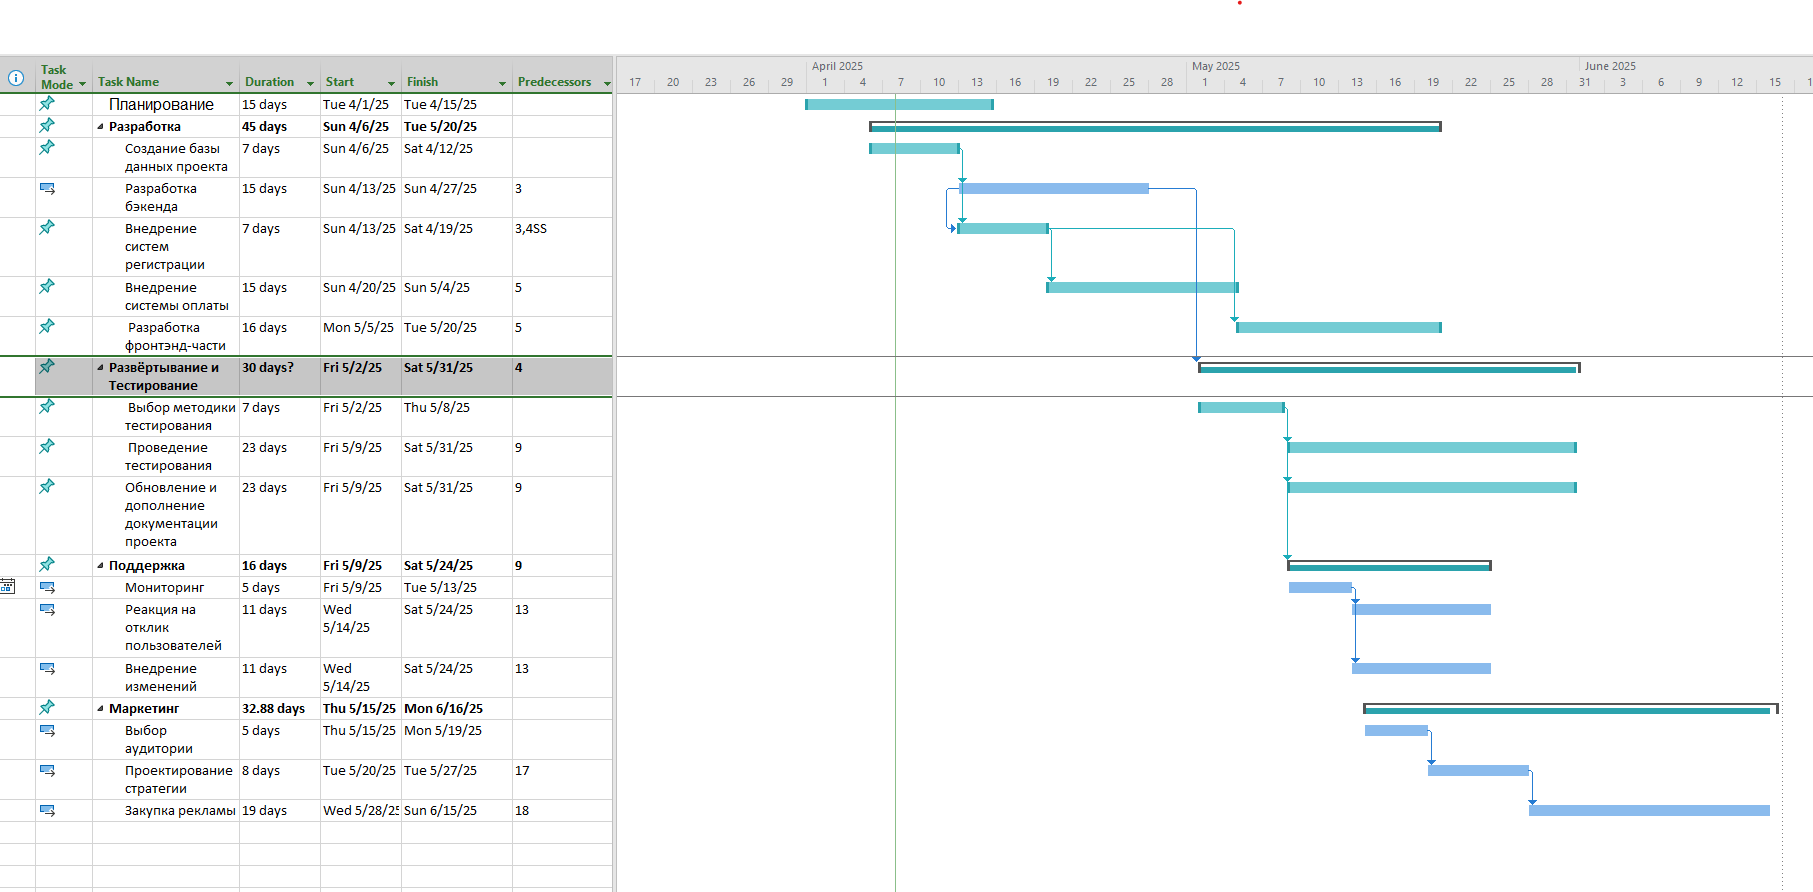
\includegraphics[width=\textwidth]{gant.png}
    \caption{Диаграмма Ганта проекта}
    \label{fig:gantt}
  \end{figure}

\section{Стоимость проекта}
На основании составленного WBS и предполагаемой трудоёмкости, были оценены сроки реализации и стоимость проекта.

\begin{itemize}
    \item \textbf{Продолжительность}: порядка \textbf{45 рабочих дней} (6–9 недель), с учётом частичной параллельности задач. Диаграмма Ганта построена в соответствии с этапами WBS.
    \item \textbf{Стоимость реализации} (при средней ставке \$20/час):
    \begin{itemize}
        \item По экспертной оценке: \textbf{\$16,400}
        \item По методу UCP: \textbf{\$26,460}
    \end{itemize}
\end{itemize}

Полученные данные могут быть использованы для формирования бюджета и распределения ресурсов по этапам проекта.

\end{document}
